\documentclass[10pt,twocolumn]{article}
\usepackage{cite}
\usepackage{amsmath,amssymb,amsfonts}
%\usepackage[full]{textcomp}
%\usepackage{fdsymbol}
%\usepackage{newtxtext,newtxmath}
\usepackage{multicol}
\setlength{\columnsep}{0.75cm}
\usepackage{caption}
\usepackage{graphicx}
\usepackage{csquotes}

\def\BibTeX{{\rm B\kern-.05em{\sc i\kern-.025em b}\kern-.08em
    T\kern-.1667em\lower.7ex\hbox{E}\kern-.125emX}}
\usepackage{hyperref}
\usepackage[margin=1.75cm]{geometry}

%\graphicspath{{img/}}

\title{Optimized Payment Execution and Planning Strategy for the Lightning Network}


\begin{document} 

\author{Rene Pickhardt}

\maketitle

 
\begin{abstract}
lets go
\end{abstract}

%==========================================================================
\section{Introduction}

\section{Mathmatical background}
Let $a\in\mathbb{N}$ be the amount that is supposed to be delivered from a sending node to a receiving node on the Lightning Network.
We define the weithed directed Graph $G_a = (V,E_a)$. 
$V$ is the set of vertices and $E\subset V\times V \times \mathbb{R}_+$ the set of edges with the weight as the third component.
Given two nodes $v_i$ and $v_j$ an edge $e_{i,j}=(v_i,v_j,l_{i,j})$ in this graph exists if and only if there is a payment channel between the nodes $v_i$ and $v_j$.
Let $P_{i,j}(X\geq a)$ be the channel success probability for a payment of amount $a$ from node $v_i$ to $v_j$.
Note that due to some knowledge that nodes learn during the payment process $P_{i,j}(X\geq a) \neq P_{j,i}(X\geq a)$ even though equality might hold initially for many edges.
Then the value $l_{i,j}$ encodes the negative log probability $l_{i,j} = - log(P_{i,j}(X\geq a))$ that the amount $a$ can successcully be forwarded from node $v_i$ to node $v_j$.
If $P_{i,j}(X\geq a) = 0$\footnote{for example because $a$ is larger than the channel capacity} instead of setting $l_{i,j}=\infty$ we remove the edge.
If the probability takes the value $1$ and routing ability is certain we set the weight to $0$ as defined by the logarithm and keep the edge.

Given a sender $s \in V$  and a destination $d\in V$ the solution of the Dijkstra algorithm from $s$ to $d$ produces the $(s,d)$-path $\pi_{s,d}$ with the highest likelihood to deliver the payment with the amount $a$.\footnote{do we need a reference or proof or is that clear?}\footnote{it woul be nice to proof that for $a'<a$ the path will not change. However I believe this is not possible. Imagine an artificial graph where one has high capacity edges s-->b-->c-->r and a low capacity edge s-->r. if the amount is sufficiently small s-->r will have higher probability. Maybe move this to the appendix.}
The success probability $p_{s,d}$ of the path $\pi_{s,d}$ can be computed by:
\[
p_{s,d} = \exp\left(-\sum_{l_{i,j}\in \pi_{s,d}}l_{i,j}\right)
\]
we call $\delta_{s,d} = \sum_{l_{i,j}\in \pi_{s,d}}$ the log distance of the path $\pi_{s,d}$.

Assuming we have $k$ disjoint $(s,d)$-paths $\pi_1,\dots,\pi_k$ with corrsponding log distances $\delta_1,\dots,\delta_k$ we can express the success probability of the $k$-part payment\footnote{instead of using multipart payment and the abbrivation mpp and talk about $k$-mpp or mpp of size $k$ we suggest to say a $k$-part payment and use the abbrivation kpp if we talk an mpp with a fixed value of $k$.} as
\[
p_{s,d} = \exp\left(-\sum_{i=1}^k\delta_i\right)
\]
Note that the log distance $\delta_i$ will in most cases depend on the amount that was sent over the path $\pi_i$.
A $k$-split of the payment amount $a$ is a collection of of positive integers $a_1,\dots,a_k \in \mathbb{N}$ such that $\sum_{i=1}^ka_i=a$.
Recall that $\exp$ is a group homomorphism from the addive group of real numbers to the multiplicative group of real numbers which is why we can write: 
\[
p_{s,d} = \prod_{i=1}^k\exp(-\delta_i)
\]
realizing that the $\delta_i$ are sums again we can even go further and write:
\[
p_{s,d} = \prod_{i=1}^k\left(\prod_{l_{v,u}\in\pi_i}\exp(-l_{v,u})\right)
\]
replacing the log probabilities the exponential function and logarithm cancle out so that we get
\[
p_{s,d}(a_1,\dots,a_k) = \prod_{i=1}^k\left(\prod_{l_{v,u}\in\pi_i}P_{v,u}(X\geq a_i))\right)
\]
which is a function $p_{s,d}:\mathbb{R}^k_+\longrightarrow\mathbb{R}_+$ and depends only on the fixed channel success probabilities and the $k$-split of the amount $a$ which serves as a constraining condition.
We can thus compute the maximum probability by solving the optimization problem using the method of Lagrange multipliers.
.
\subsection{Example using uniform distributions}
for a payment channel with capacity $c_{v,u}=c_{u,v}\in\mathbb{N}$ we can easily compute the channel succes probability as:
\[
P_{v,u}(X\geq a)=\frac{c_{v,u}+1 - a}{c_{v,u}+1}
\]

Given the following Lightning Network in figure \ref{fig:example_LN}
\begin{figure}[htpb]
  \center
  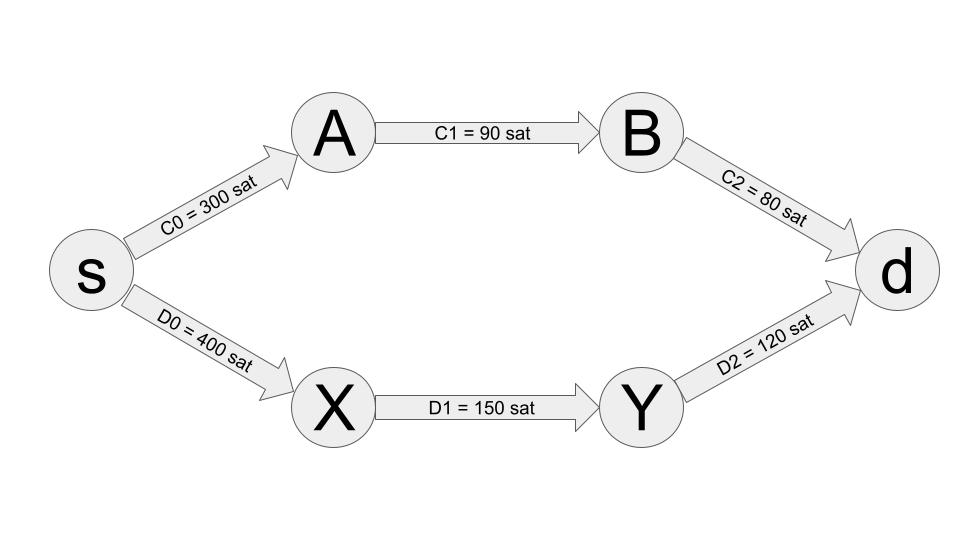
\includegraphics[width=0.45\textwidth]{img/example_LN.jpg}
  \caption{An example Lightning Network in which two paths from $s$ to $d$ exist. Note that we assume that for any given payment amount the first edge has enough liquidity and no uncertainty.}
  \label{fig:example_LN}
\end{figure}
The probability function $p_{s,d}(a_1,a_2)$ for a $2$-split $a=a_1+a_2$ of the amount $a$ is given by:
\[
\frac{c_1+1 - a_1}{c_1+1}\cdot\frac{c_2+1 - a_1}{c_2+1}\cdot\frac{d_1+1 - a_2}{d_1+1}\cdot\frac{d_2+1 - a_2}{d_2+1} 
\]
Note that this is a polynomial of degree $4$ which corresponds to the number total number of channels with uncertain balance in the $k$-split of the payment.
Also note that the probability for the first hope is set to $1$ as the sending node would only use paths for which the local channel has enough balance to make a payment.\footnote{later in the paper we will actually depending on success of failur of payment attempts update the probabilities of edges.}
The Lagrange function $\mathcal{L}$ of the corresponding optimization problem is defined as:
\[
\mathcal{L}(a_1,a_2,\lambda)=p_{s,d}(a_1,a_2) - \lambda\cdot(a_1+a_2-a)
\]

The gradient $\nabla\cdot\mathcal{L}$ computes as:

\[
    \nabla\cdot\mathcal{L} := \begin{bmatrix}
           \frac{\partial\mathcal{L}}{\partial a_1} \\
           \frac{\partial\mathcal{L}}{\partial a_2} \\
           \frac{\partial\mathcal{L}}{\partial \lambda}
    \end{bmatrix}  \stackrel{!}{=}
    \begin{bmatrix}
           0 \\
           0 \\
           0
    \end{bmatrix}
\]
As it needs to be set equals zero it gives rise to a set of $3$ non-linear eqautions in three varables $a_1,a2,\lambda$.
The equaions are actually polynomials of degree $3$ which is one less than the degree of $p_{s,d}$.
Solving the system of equations for any payment amount $a$ produces the following optimal values for $a_1$ and $a_2$ which are depicted in figure \ref{fig:optimal_split_example}
\begin{figure}[htpb]
  \center
  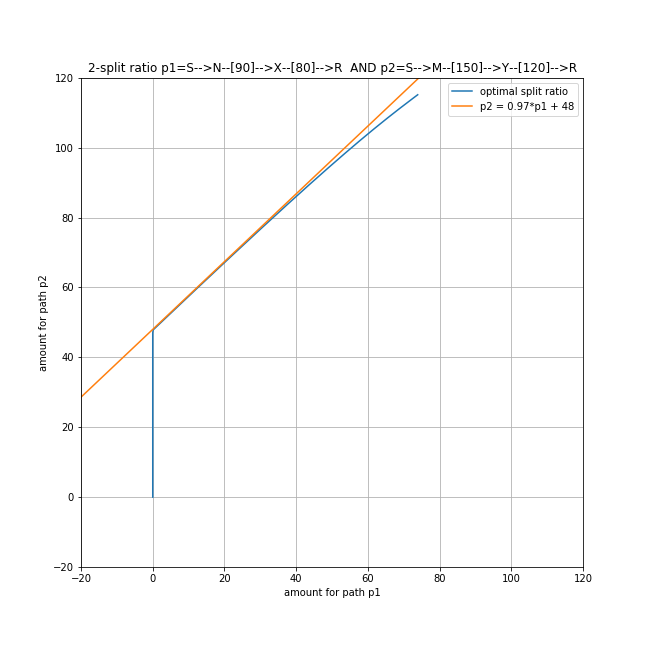
\includegraphics[width=0.45\textwidth]{img/optimal_split_example.png}
  \caption{We can see that for values lower than 48 satoshi no split is recommended as it is most likely to complete the payment in a signle payment over the lower of the two paths. After that the split ratio is almost constant as can be see via the straight line $a_2=0.97a_1 + 48$}
  \label{fig:optimal_split_example}
\end{figure}

By the theory we already know that for smaller amounts that we wish to conduct the probability of delivering the payment increases.
Nevertheless we depicted the results for some concrete values of $a$ in figure \ref{fig:optimal_split_example_amounts}

\begin{figure}[htpb]
  \center
  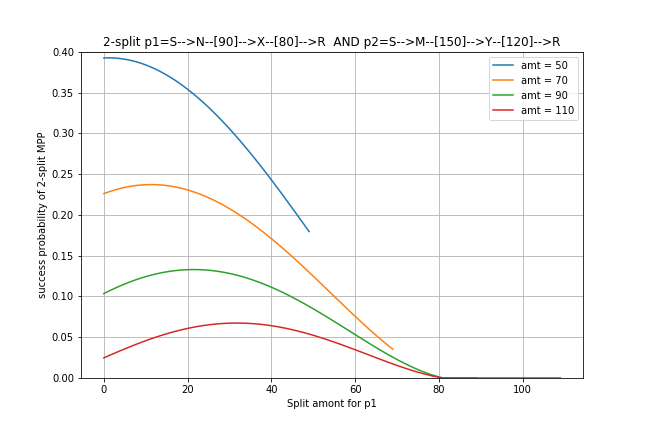
\includegraphics[width=0.45\textwidth]{img/optimal_split_example_amounts.png}
  \caption{Note that the maxium value that is supposed to go to path $p_1$ defines the amount for $p_2$ by $a2=a-a_1$ and the values relate to the theory.}
  \label{fig:optimal_split_example_amounts}
\end{figure}


%Fixing $k$ $(s,d)$-paths and assigning each path the amount $a_i$ of the $k$-split we want to decide which split maximizes the probability $p_{s,d}$.

%Given $a$ we wonder how to choose an $n$-split of $a$ so that the payment reliability is maximized.\footnote{one proxy for that could be to minimize the expectation value of attampts. However given the fact that we have concurrency in reality this might not be the best proxy. Maximizing the Likelihood is inverse to the expectation value and thus also potentially not the best metric. If we can't coming up with something better we need to focus on this metric as a proxy.}

%\subsection{Single channel and single path}
%Let $P(X \geq a)$ be the channel success probability for a payment of size $a$.
%Further $a_1,a_2$ be two positive numbers such that $a=a_1+a_2$. 
%Let us assume $a_1$ was delivered successful.
%We can now update the prior probability and compute the likelihood for $a_2$ to be delivered.



\section{Results}

\section{next steps}
\begin{itemize}
\item implementing and describing the general case (n-split) on actual lightning network data that is based on solving the optimization problem with lagrange multipliers. (shall we use an arbitrary probability distribution as a prior or shall we use uniform distributions? I guess to describe the problem we can use arbitrary distributions and for the solution we can compute this with uniform priors.)
\item Understand if the solution to the non linear system of equation that arises from the lagrange multipliers can efficiently be approximated well enough (for example taylor approximation!) and quantify the loss in effectiveness in comparison to gain in computational complexity.
\item define a proper experimental setup strategy (probably using proper sampling of payment pairs and amounts)
\item solve the candidate selection process (e.g. take highest likely path with full amount reduce capacities by the amount and select next probable path (this allows for non disjoint paths) or remove that path completely (this allows for disjoint paths)) both strategies are obviously only an approximation to path selection. But it is infeasble to take \textit{all} paths and solve the problem on subsets.\footnote{maybe neglect this until next paper it seems to me a different modelling approach of the problem would have to be taken. not sure if we can solve this and it seems all the other stuff is already pretty dense}
\item adopt the problem to non disjoint problems
\item define the payment planning and execution algorithm. I currently have the following in mind:
  \begin{enumerate}
  \item generate $n$ candidate paths and rank them by likelihood (with one of the two mentioned strategies and the dijkstra search on the minus-log-prob weighted graph arising from previous research).
  \item solve the optimal split for the top $k$ paths according to the exact math (or approximation if feasable).
  \item concurrently make attempts of the $k$ split with the highest overall success probability.
  \item after the first failed attempt wait a timeout to collect more failures and solve the problem for the residual amount by first updating the probabilities via the learnt information and then repeat from step one. (In later repitation include any failed onions from all previous rounds)
  \item do this for $x$ rounds or until the graph does produce splits with sufficiently high probabilities anymore. 
  \end{enumerate}
\item Test how quickly (after how many rounds) we know for sure that we cannot find a path! or at least that the success probability drops to a certain amount! this can be the basis for an adaptive strategy for the number of rounds. e.g. we can say that we do not want to try if the success probabilty goes below $p$ or we don't do more rounds. In this way we can very precisly define service level agreements.
  \item include the optimal local splitting strategy to optimize channels towards the gini coefficient of the imbalance paper \cite{Pickhardt2019}. (while this will decrease the success probability it might over all improve the network as channels become normally distributed) we can simulate the effect of that change a) on a local level but also b) if everyone implements this!
\end{itemize}

\subsection{newer thoughts after running examples}

\begin{enumerate}
\item Maybe it is possible to get rid of candidate path generation.
We could use a very large $k$-split over \textit{all} paths and adopt the optimization problem to not allow negative amounts or amounts larger than channel or the amount to send.
This could yield a solution of the $k$ split in which $l\leg k$ variables are zero in the optimal solution as the solution is on the border of the constrained problem.
\item With regard to splitting strategies we could write down probabilities for equidistant split, the optimial split and the start split before the optimization problem (which is proportional to the smallest channel across each path).
\item I think it was mentioned before but especially when following through the first idea we have to account for non disjoint paths.
\end{enumerate}

Conclusion: I think there is a reasonable chance to formulate this problem as a global optimization problem.
  

\subsection{Thoughts after phone call}
\begin{enumerate}
\item It is rather easy to drop the disjoin path assumption in candidate selection. if two paths with amounts $a_1,a_2$ share the capacity $c$ edge we take $\frac{c+1-a_1-a_2}{c+1}$ into account instead of $\frac{c+1-a_1}{c+1}\cdot\frac{c+1-a_2}{c+1}$
\item We suspect that the round based algorithm will actually be able to decide the flow problem. However we are not sure if we can formally proof completeness. In case we find a counter example it would be good to have an empirical evaluation how often the algorithm tends to decide the flow problem correctly.
\item With respect to metrics. Success means a correct decision of the flow problem. That should be 100\% or at least quantifilable. What we are interested in is how quickly is the decision found? 
\item Another \textit{shower thought}: Respecting routing fees would actually result as a nother contrain to the optimizing problem
\end{enumerate}

\bibliography{mppSplitting}
\bibliographystyle{plain}


%\end{multicols}
\end {document}
